\chapter{Detecting exoplanets with the radial velocity method}

%todo review sinusoidal curves and how to extract info from curve fits

%todo remove unneeded equations, like 

%todo add equation for 2\pi r / T for orbital velocity

% TA will demonstrate two hanging masses on a ruler, which is balanced on a horizontal rod mounted on a support stand. The masses should be very uneven to simulate a star and planet. Demonstrate how the center of mass changes with the change in separation and change in mass of the planet.

%todo maybe change data to start at t=0 to make period scaling more intuitive?

%todo clarify semi-major axis - is it of the planet, or star? Consider changing to "radius", since we are assuming circles everywhere

\section{Introduction}

\begin{figure}
	\centering
	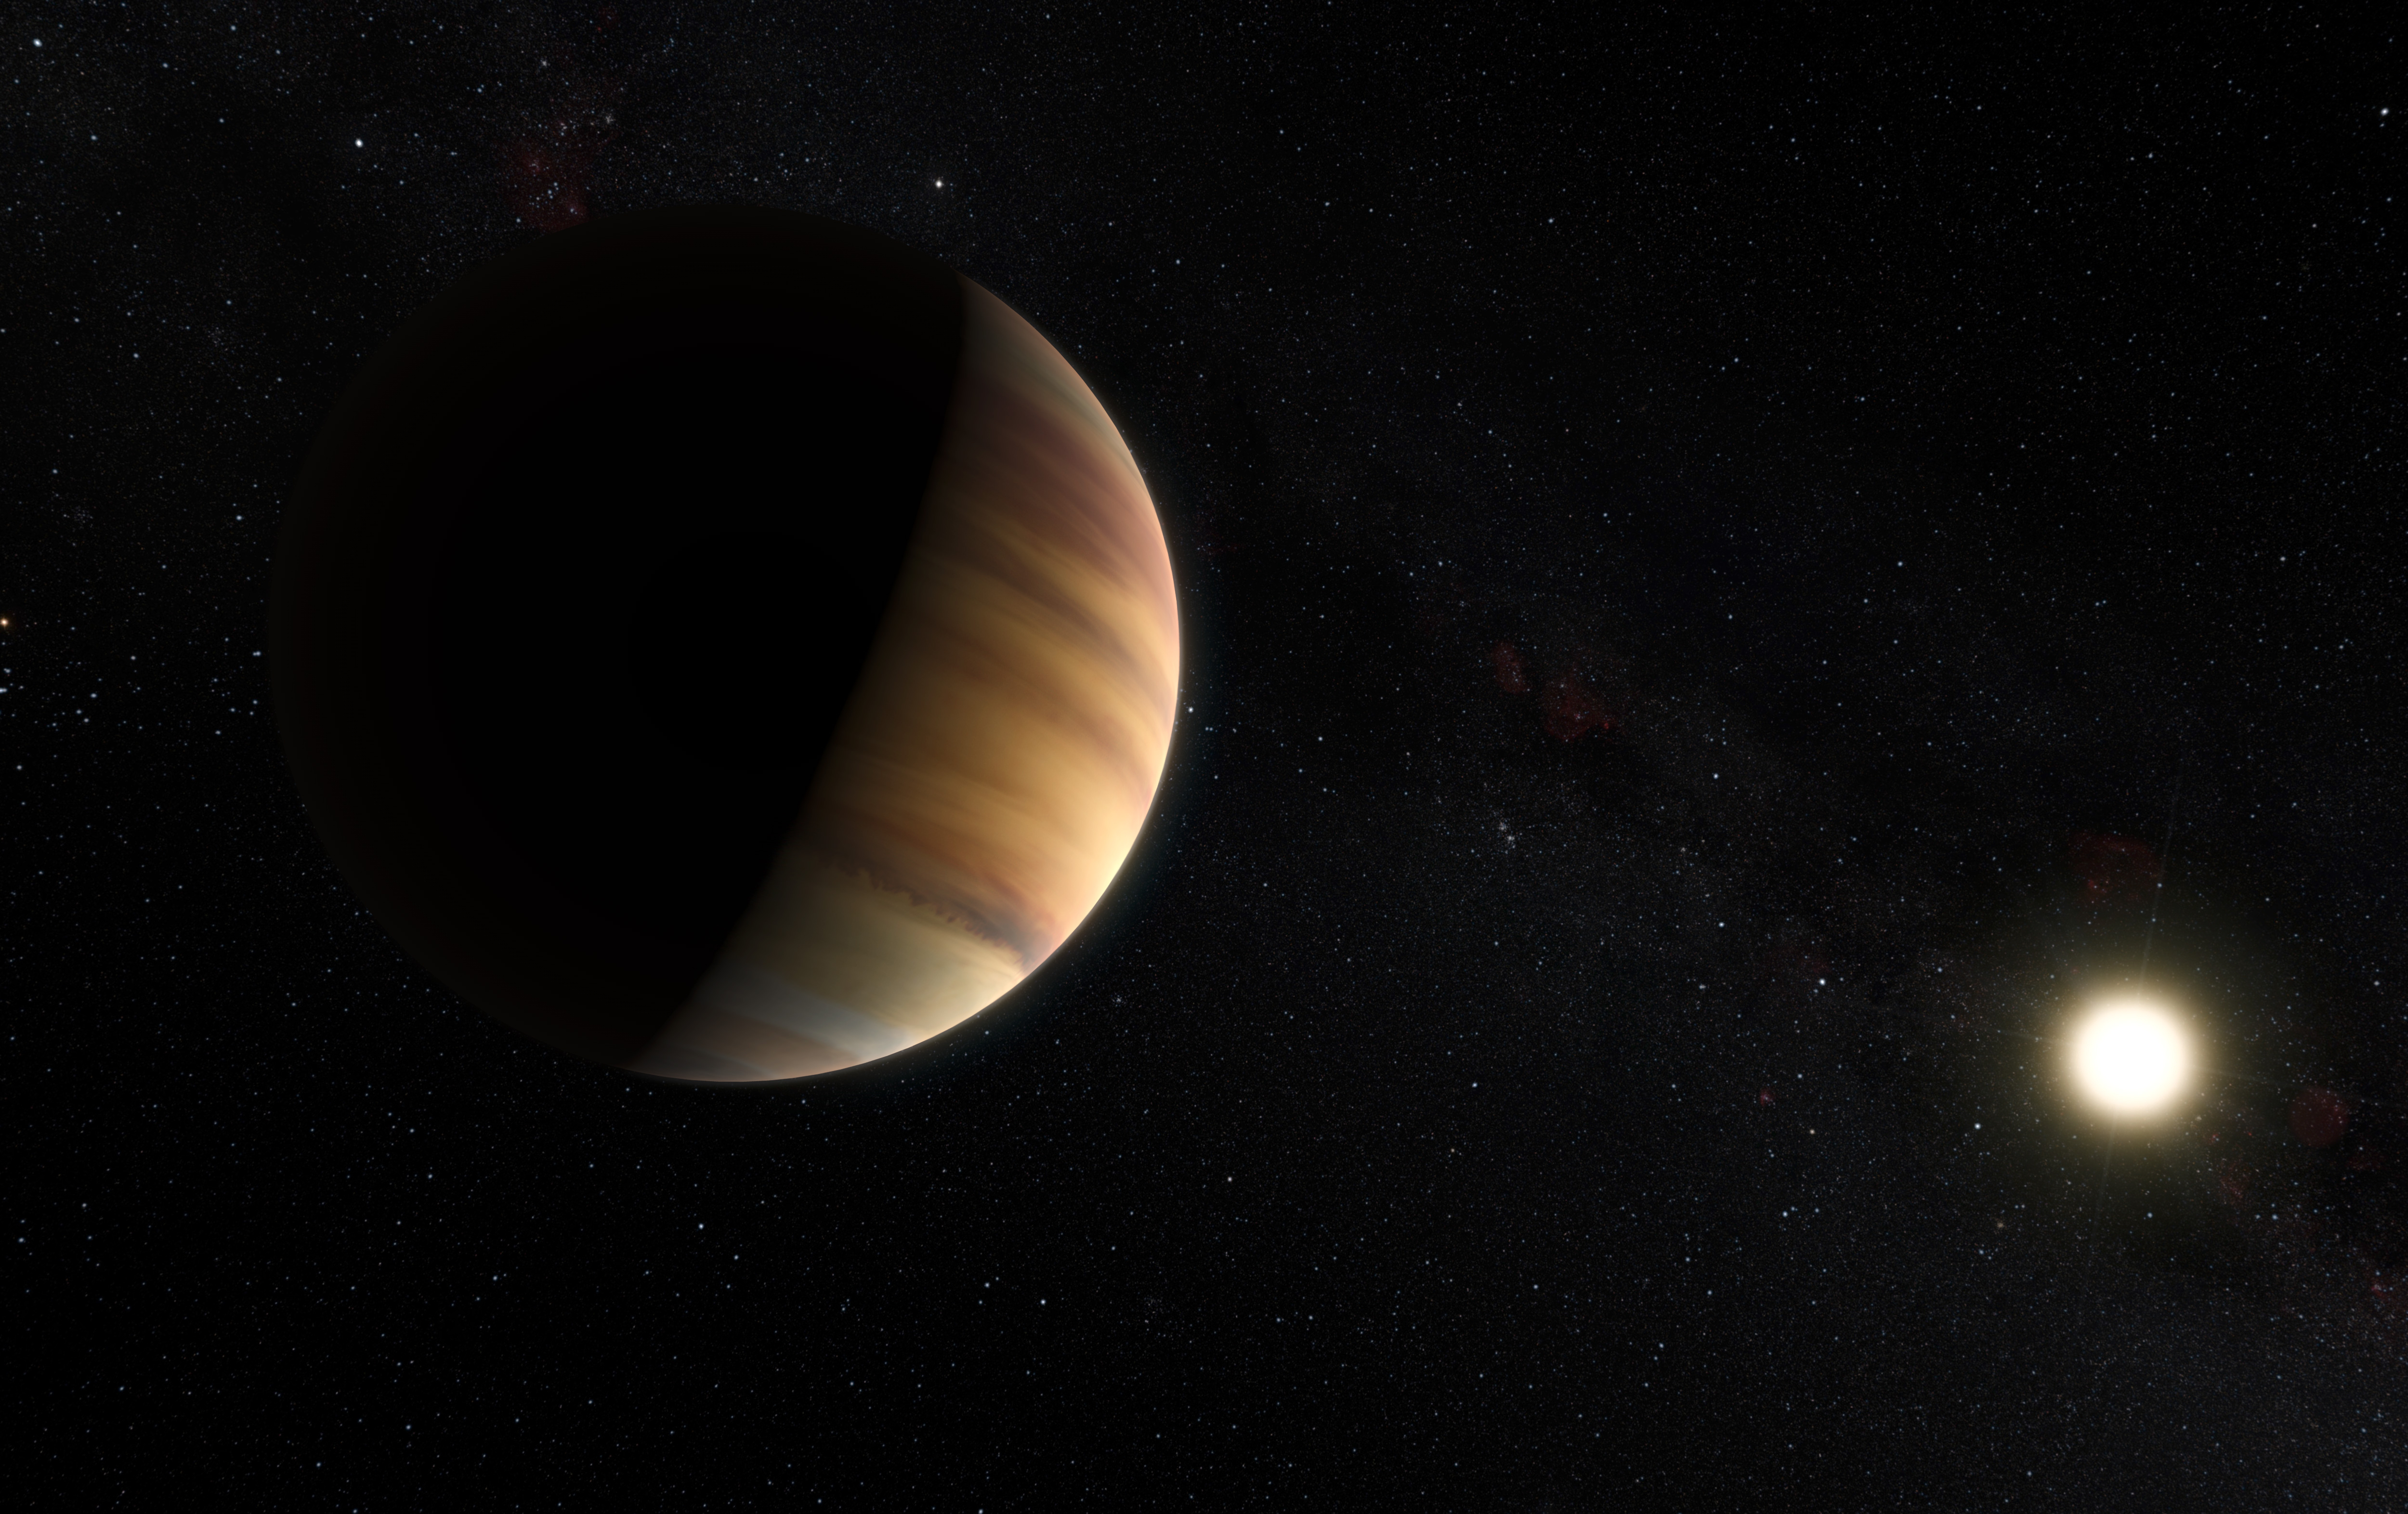
\includegraphics[width=0.9\textwidth]{radial-velocity/ArtistImpression_51PegB}
	\caption{Artist impression of the hot Jupiter exoplanet 51 Pegasi b, the first exoplanet found arround a normal star. (Source: ESO)}\label{rv:fig:artist-51pegb}
\end{figure}

In the Fall of 1995, two Swiss astronomers announced evidence for a planet orbiting the star 51 Pegasi, a groundbreaking discovery since the star, 51 Pegasi, is very similar to our own Sun. Since 1995, thousands of potential exoplanets have been detected and the field of exoplanet science has become a pillar of modern astronomy.

In this lab, we will explore the radial velocity technique, the method used to detect the first exoplanets and a powerful technique for studying exosolar planetary systems.

%\subsection{Grading}

%Each bolded instruction is worth 4 points, and each numbered question is worth 2 points. We include 10 points for attendance and participation to arrive at 60 points for this lab.

\section{Team roles}

\begin{steps}
	\item \textbf{Decide on roles} for each group member.
\end{steps}

The available roles are:
\begin{itemize}
	\item Facilitator: ensures time and group focus are efficiently used
	\item Scribe: ensures work is recorded
	\item Technician: oversees apparatus assembly, usage
	\item Skeptic: ensures group is questioning itself
\end{itemize}

These roles can rotate each lab, and you will report at the end of the lab report on how it went for each role. Some members will be holding more than one role. For example, you could have the skeptic double with another role. Consider taking on a role you are less comfortable with, to gain experience and more comfort in that role.

Additionally, if you are finding the lab roles more restrictive than helpful, you can decide to co-hold some or all roles, or think of them more like functions that every team needs to carry out, and then reflecting on how the team executed each function.

\section{Add members to Canvas lab report assignment group}

\begin{steps}
	\item On Canvas, navigate to the People section, then to the ``Groups'' tab. Scroll to a group called ``L2 Radial [number]'' that isn't used and have each person in your group add themselves to that same lab group.
\end{steps}

This enables group grading of your lab report. Only one person will submit the group report, and all members of the group will receive the grade and have access to view the graded assignment.

\section{Building Intuition}

We usually say that a planet orbits a star, but this isn't quite true --- both planet and star orbit the center of mass of the system. This is called the \textit{barycenter}. This results in the star wobbling in a circular motion. The motion is too small to detect from Earth directly. But when the source of waves moves towards or away from an observer, the wavelength of that wave is shifted lower or higher, respectively. Since stars have characteristic gaps in the spectrum of light they emit, we can detect this \textit{Doppler shift}, and thus determine the \textit{radial velocity} of the star. From this and our knowledge of orbital dynamics, we can deduce characteristics of exoplanets orbiting that star.

\begin{steps}
	\item Open the link for the Center of Mass webpage (\url{https://astro.unl.edu/mobile/center-of-mass-simulator/index.html}). Use the sliders to explore how varying separation and relative mass changes the Center of Mass.
	
	\item Open the link for the radial velocity simulator (\url{https://www.bu.edu/astronomy/visualizations/AlienWorlds/simulation-radial.html}).
		
	\item Vary the mass of the planet, the mass of the star, and the distance. Note how the radial velocity graph changes. Vary the other parameters (viewing angle, star radius, planet radius) and see how the radial velocity changes. \textbf{Include your findings in your report.}		
\end{steps}

\section{Building quantitative intuition}

For this lab, the following values will be useful:
\begin{itemize}
	\item $1\:\textrm{AU} = 1.496 \times 10^{11}\:$m (approximate distance between the Earth and the Sun)
	
	\item $1\:\textrm{M}_\textrm{J} = 1.898 \times 10^{27}\:$kg (mass of Jupiter)
	
	\item $1\:\textrm{M}_\textrm{Sun} = 1.989 \times 10^{30}\:$kg (mass of the Sun)
	
	\item $G = 6.674 \times 10^{-11}\:\mathrm{N}\:\mathrm{m}^2/\mathrm{kg}^2$ (Newtonian constant of gravitation)
\end{itemize}

\subsection{Mathematical tools for orbital mechanics}

Equation for finding the center of mass position $x_\mathrm{CM}$ for two masses, $m_1$ and $m_2$, at positions $x_1$ and $x_2$:
\begin{equation}
 x_\mathrm{CM} = \frac{m_1 x_1 + m_2 x_2}{m_1 + m_2}
\end{equation}

An object in a circular orbit of radius $r$ experiences an acceleration $\vec{a}$ directed inward with magnitude
\begin{equation}\label{rv:eq:circular}
 a = \frac{v^2}{r} \,.
\end{equation}
In our case, the object is experiencing this acceleration as a result of the force exerted on it through gravity by the other object according to
\begin{equation}\label{rv:eq:grav}
 F = G \frac{m_1 \: m_2}{r_{12}^2} \,,
\end{equation}
where $r_{12}$ is the distance between the two objects, which is different from the orbital radius, since the object orbits the center of mass (or barycenter), rather than the other object.

To relate velocity in the first equation with the masses of the objects in the second equation, we can use the fact that the acceleration that an object experiences is proportional to the force on it and inversely proportional to its mass --- or in equation form,
\begin{equation}\label{rv:eq:n2l}
 a = \frac{F}{m} \,,
\end{equation}
also known as Newton's second law of motion.

So in this equation, if we substitute in $a$ from Eq. \ref{rv:eq:circular} and $F$ from Eq. \ref{rv:eq:grav}, we can solve for the orbital velocity of Object 1 like so:
\begin{eqnarray}
 \frac{v_1^2}{r_1} &=& \frac{G \frac{m_1 \: m_2}{r_{12}^2}}{m_1} \\
 \frac{v_1^2}{r_1} &=& G \frac{m_2}{r_{12}^2}
\end{eqnarray}
These ideas should be familiar from assignment 2. 

\subsection{Analyzing a sample orbital system}

Consider the picture in Figure~\ref{rv:fig:two-body-cm} and define $M_\textrm{p} = 0.5 M_\textrm{J}$ as the mass of the planet (the smaller object),  $M_\textrm{S} = 1.0 M_\textrm{Sun}$ as the mass of the star (the larger object), and $r_{12} = 0.0527\:$AU be the separation between the two. Assume the system is in a circular orbit.

\begin{figure}
	\centering
	\includegraphics[width=0.4\textwidth]{radial-velocity/two-body-cm}
	\caption{Schematic of a star (upper-left) and planet (lower-right) orbiting a common center-of-mass (marked with a red cross).}\label{rv:fig:two-body-cm}
\end{figure}

\begin{steps}
	\item How far is the Center of Mass from the center of the star (in AU)?
	
	\item What is the star’s orbital radius, $r_1$ (in AU)?
\end{steps}

Since the star is moving around the Center of Mass, it has a non-zero velocity. Let the orbital period of the system be $P = 4.42\:$days.

\begin{steps}
	\item What is the orbital velocity of the host star?
	
	\item Sketch the figure, then on that sketch, draw arrows showing the velocity at different parts of the orbit. What happens to the direction of the star’s velocity as the planet traces out its orbit?
\end{steps}

Astronomers can use spectroscopic techniques for measuring the velocity of stars along the line of sight between the earth and the star. In the illustration in Figure~\ref{rv:fig:two-body-cm}, suppose the earth is to the right of the system so that we are observing the system edge on from the right side of the page. 

\begin{steps}
	\item \textbf{Draw a graph} similar to Figure~\ref{rv:fig:graph} and then draw on it the ``line of sight'' velocity for the star as a function of time (hint: it will be a trigonometric function).
\end{steps}

\begin{figure}
	\centering
	\includegraphics[width=0.6\textwidth]{radial-velocity/radial-graph}
	\caption{Graph to draw for radial velocity estimation.}\label{rv:fig:graph}
\end{figure}

\begin{steps}
	\item How are the period and amplitude related to the orbital period and the star’s velocity?
\end{steps}

Next, consider a similar system only with a planet that is twice the mass ($M_\textrm{p} = M_\textrm{J}$, $M_\textrm{S} = M_\textrm{Sun}$, $d = 0.0527\:$AU, and $P = 4.42\:$days).


\begin{steps}
	\item What is the system's host star orbital radius (in AU) and orbital velocity (in m/s)?
	
	\item How do these compare with the values for the previous system with a less massive planet?

	\item \textbf{Sketch the line of sight velocity} for this more massive system on the same plot that you already drew.

	\item How does the line of sight velocity depend on the planet’s mass?
\end{steps}

\section{Radial velocity of 51 Peg}

Table~\ref{rv:tab:51peg} lists measured line of sight velocities for the star 51 Pegasi measured by Marcy \& Buttler in 1995 at the Lick Observatory in California. You will use this data to determine the mass and orbital distance of the exoplanet orbiting 51 Peg.

\begin{table}
	\centering
	\includegraphics[width=\textwidth]{radial-velocity/51-peg-velocities}
	\caption{Line-of-sight velocities for 51 Pegasi measured over time.}\label{rv:tab:51peg}
\end{table}

\begin{steps}
	\item Open the Google Sheet found here: \url{https://docs.google.com/spreadsheets/d/1aTp-UxxgGf3wzgCrGr6HHANdEkvuTbgkLRbQcpRHDGQ/edit?usp=sharing}
	
	\item Make a copy of this sheet for your group to use.
\end{steps}

This spreadsheet contains the data in Table~\ref{rv:tab:51peg}, as well as a model for the velocity as a function of time. Circular motion, projected to 1 dimension, can be described by a sine function. The most general sine function has free parameters that can be changed to represent any sinusoidal motion. For example, the velocity function can be described with
\begin{equation}
 v(t) = \textrm{A} \sin \left[\frac{2 \pi}{\textrm{B}}\left(t + \textrm{C}\right)\right] + \textrm{D} \,,
\end{equation}
where A is the amplitude of the motion and B is the period of the motion. C is a time offset, to account for where the star is in its oscillation cycle at $t=0$. D is constant velocity offset, to account for any constant line of sight velocity that was not already compensated for (for example, the observer's motion with respect to the barycenter of the exoplanet system).

%Use the free software SciDAVis to plot this data. You can download and install it on your computer from \url{https://sourceforge.net/projects/scidavis/}.
%, or you can use the lab computers, which have it installed already.

%\begin{framed}
%\textbf{Mac users:} if you get an error when trying to run SciDaVis, saying that it is from an unidentified developer, follow the directions at the following website to let it run:
%
%\url{https://support.apple.com/guide/mac-help/open-a-mac-app-from-an-unidentified-developer-mh40616/10.15/mac/10.15}
%\end{framed}

\begin{steps}
	\item In your copy of the spreadsheet, explore changing the fit parameters A--D and see what effect it has on the model velocity.
	
	\item For your first pass at fitting the model, find a set of parameters that makes the model velocity curve visually similar to the data.
\end{steps}

To get a more precise estimate for the parameters, you can use a common statistic called the \textit{rms deviation}. "rms" stands for root-mean-square. For $N$ data points $y_{\textrm{data},i}$, the rms deviation from the theoretical model points $y_{\textrm{model},i}$ can be found by
\begin{equation}
 \textrm{rms deviation} = \sqrt{\dfrac{\sum_{i=0}^{N-1} \left( y_{\textrm{data},i} - y_{\textrm{model},i} \right)^2}{N}} \,.
\end{equation}
The smaller the rms deviation, the closer the fit. The rms deviation is already calculated for you in cell \texttt{D6} in the spreadsheet.

\begin{steps}
	\item Starting with your first pass estimate of parameters, vary them to minimize the rms deviation and find your best fit parameters. \textbf{Record these parameters, the resulting plot, and your final rms deviation.}
\end{steps}

%Then, fit an equation to the data. To do so in SciDAVis, first save the project, so you won't accidentally lose your work. Then, select Analysis $\blacktriangleright$ Fit Wizard... from the drop-down menu. Type your desired equation into the large box. You can use any of the functions you can find in the lists at the top of the window and combine them how you would like. For fit parameters, use the letters a, b, c, and so on. For each fit parameter you use, include it in the list of parameters. For example, if you think the data are best represented by a tangent function, you could put ``\texttt{b*tan(c*x+d)}'' in the box. Then click the ``Fit $>>$'' button, then the ``Fit'' button to fit the data with this equation. This finds the parameters for the equation that make it best fit the data. Experiment to find an equation that seems to fit well.
%
%You can retrieve the fit parameters and their uncertainties from the Results Log on the main window. \textbf{Include the graph, the fit parameters, and their uncertainties in your report.}

\begin{steps}
	\item From your fit to the data, what is the orbital period (days) and host star orbital velocity (m/s) -- assuming the planetary orbit is edge-on so the radial velocity amplitude equals its full velocity?
	
	\item What is the orbital radius (in AU) for the host star?
\end{steps}

Kepler's third law relates the orbital period to the system's semimajor axis. In the case where the planet’s mass is much smaller than the star’s mass, Kepler's third law is
\begin{equation}
 P^2=\frac{4 \pi^2}{GM} a^3 \,,
\end{equation}
where $P$ is the orbital period, $G$ is Newton's constant, $M$ is the mass of the star, and $a$ is the semimajor axis. The mass of 51Peg is $1.1 M_\textrm{Sun}$.

\begin{steps}
	\item According to your fitted orbital period and Kepler's third law, what is the system's semimajor axis?
\end{steps}

The host star orbital radius and the semimajor axis are related by the Center of Mass.

%todo clarify that they should use CoM equation, rather than K3L, since we need to not neglect the planet mass to find it.

\begin{steps}
	\item Using the system's semimajor axis, the host star radius, and the mass of 51Peg, determine the planet’s mass (in units of $M_\textrm{J}$). Of course, we really mean its minimum mass, $m \sin i$, due to the assumption of an edge-on orbit. 
\end{steps}

\section{Radial velocities for other systems}

\begin{steps}
	\item Go to the webpage for SystemicLive (\url{http://www.stefanom.org/systemic-live/}). Note that while the graphics within the tutorial are currently not visible on the website, the data visualization and analysis software are still functional.
	
	\item Click ``Open Systemic'' to start the program. Then on that first page, scroll down to ``Tutorials and Resources'' and click on the link ``51 Pegged: Rediscovering the first exoplanet with Systemic Live''.
	
	\item Follow the steps of that tutorial to analyze radial velocity data for 51Peg.
\end{steps}

Note that one key analysis tool you will use in the remainder of the lab is the power spectrum of the radial velocity data. Any periodic function from the sum of sinusoids of different frequencies and phases: that's why Ptolomy's mechanics of epicycles could fit the motion of the planets so well! The power spectrum tells us which frequencies {\itshape dominate} that decomposition. Therefore, peaks in the power spectrum correspond to periodicities in the data, and hence point to possible planetary periods in the radial velocity measurements, with smaller peaks being attributable to noise.

\begin{steps}
	\item How do the mass and separation results from Systemic compare with your earlier 51Peg numbers? Print out a plot of the ``Phased Radial Velocity'' and write on it the Period and Mass for the system.
	
	%todo be clear about how many planets to find with these ones
	%todo "screenshot", not print out plots
	\item Use Systemic to determine orbit parameters for the following systems: 47Uma, 70Vir. Print out plots for your ``Phased Radial Velocity'' for each system. Write on your plots the Period and Mass for each system orbit.
	
	\item Use Systemic to analyze the data for the Upsilon Andromedae system (noted as ``upsand''). Hint, there are multiple planets for this system. How many planets do you find? What are their masses and orbital periods?
	
\end{steps}

\section{Reflection}

Do some research on the history and background of the systems you analyzed (51Peg, 47Uma, 70Vir, and upsand). Write a one paragraph summary of this lab and discuss the following:

\begin{steps}
	\item What was the historical context and significance of these measurements?
	
	\item How do they relate to what you did in this lab?
\end{steps}

\section{Report checklist}

%Include the following in your lab report. See Appendix~\ref{cha:lab-report-format} for formatting details. Each item below is worth 10 points.
Include the following in your lab report. See Appendix~A for formatting details. Each item below is worth 10 points.

\begin{enumerate}
	\item Discussion of how radial velocity changes based on available parameters (Step 5)
	\item Answers to Questions 6--9, including figure with sketch of velocities
	\item Graph of line of sight velocity vs time for two stars (Steps 10 and 14)
	\item Answers to Questions 11--13, 15
	\item Your plots for line-of-sight velocities and fit parameters (Steps 19--20)
	\item The exoplanet's orbital period and the host star's orbital velocity and orbital radius (Steps 21--22)
	\item The star-exoplanet system's semimajor axis and the exoplanet's mass (Steps 23--24)
	\item Orbit parameters and comparison for 3 star-planet systems (Steps 28--30)
	\item Reflection on the systems you analyzed (Steps 31--32)
	\item Write a 100--200 word paragraph reporting back from each of the four roles: facilitator, scribe, technician, skeptic. Where did you see each function happening during this lab, and where did you see gaps? What successes and challenges in group functioning did you have? What do you want to do differently next time?
\end{enumerate}
